%\documentclass[aspectratio=10]{beamer} %For normal presentation (comment otherwise)
\documentclass[aspectratio=169]{beamer} %for widescreen prestentation
\usetheme{default}%{Singapore}
\usefonttheme{serif}
\usepackage{ulem}
\usecolortheme{default}%albatross, crane, beetle, dove, fly, seagull, wolverine e beaver.
\setbeamertemplate{frametitle}[default][center]
%%%%%%%%%%%%%%%%%%%%%%%%%%%%%%%%%%%%%%%%%%%%%%%%%%%%%%%%%%%%%%%%%%%%%%%%%%%%%%%%%%%%%%%%%%%%%%%
%%%%%%%%%%%%%%%%%%%%%%%%%%%%%%%%%%%%%%EXTRA PACTAGES%%%%%%%%%%%%%%%%%%%%%%%%%%%%%%%%%%%%%%%%%%%
\usepackage[utf8]{inputenc}
\usepackage[T1]{fontenc}
\usepackage[scaled]{helvet}
\renewcommand*\familydefault{\sfdefault}
\usepackage[portuguese, english]{babel}
\usepackage[round]{natbib}
\usepackage{hyperref} 
\usepackage{tcolorbox}
\usepackage{graphicx} % Required for including images
\usepackage{graphics}
%\usepackage[dvips]{graphicx} 
\graphicspath{{images/}} % Location of the graphics files
\usepackage{booktabs} % Top and bottom rules for table
\usepackage[font=small,labelfont=bf]{caption}%specifies captions on tables and figures
\usepackage{amsfonts, amsmath, amsthm, amssymb} % For math fonts, symbols and environments
\usepackage{wrapfig} % Allows wrapping text around tables and figures
\usepackage{makeidx}
\usepackage{epstopdf}%adiciona imagens em formato eps no pdf.
\usepackage{subfigure}%cria ambientes de multifiguras
\usepackage{float}%coloca as figuras exatamente aonde você quer
\usepackage{times}
\usepackage{tikz}%pacote para fazer fluxogramas
\usepackage{epsfig}
\usepackage{graphicx}
\usepackage{epstopdf} %converting to PDF
\usepackage{verbatim}%
\usepackage{multicol}
\usepackage{xcolor}
\usepackage[makeroom]{cancel}
\usepackage[framemethod=tikz]{mdframed}
\usepackage{hyperref} 
\usepackage{smartdiagram}
\usepackage{amssymb}
\usepackage{etoolbox}
\usepackage{tikz}
\usetikzlibrary{mindmap}
\usepackage{metalogo}
%\smartdiagramset{uniform color list=gray!60!black for 6 items,
%back arrow disabled=false}
\usepackage{booktabs} % Top and bottom rules for table
\usepackage[font=small,labelfont=bf]{caption} % Required for specifying captions to 


% Configuracao das referencias
\hypersetup{
    colorlinks=true,
    citecolor=blue,   % Cor das refer\u00eancias citadas
    linkcolor=blue,   % Cor dos links
    urlcolor=blue     % Cor dos links para URLs
}

% Configurar as cita\u00e7\u00f5es com par\u00eanteses e a cor azul
\setcitestyle{round} % Par\u00eanteses ao inv\u00e9s de colchetes

% Definir cor azul para cita\u00e7\u00f5es, incluindo par\u00eanteses
%\renewcommand{\cite}[1]{\textcolor{blue}{\citet{#1}}}
%\renewcommand{\citep}[1]{\textcolor{blue}{\citep{#1}}}

%%%%%%%%%%%%%%%%%%%%%%%%%%%%%%%%%%%%%%%%%%%%%%%%%%%%%%%%%%%%%%%%%%%%%%%%%%%%%%%%%%%%%%%%%%%%%
%%%%%%%%%%%%%%%%%%%%%%%%%%%%%%%%%%%%% PREAMBLE %%%%%%%%%%%%%%%%%%%%%%%%%%%%%%%%%%%%%%%%%%%%%%%%
%\subtitle{}
\author[Victor Carreira]{} 
\title{A inteligência artificial é inteligente?}
\subtitle{Hunger of Science}
\institute{LOOP}
\date{Setembro de 2024}
\subject{Grupo LOOP}
%\setbeamertemplate{footline}[frame number]
%\setbeamercovered{transparent}
\setbeamertemplate{navigation symbols}{}
% Tela cheia
\hypersetup{pdfpagemode=FullScreen}
\usepackage{ragged2e}
%\justifying
%\addtobeamertemplate{headline}{}
\usepackage{tikz}
\usetikzlibrary{shapes.geometric, arrows}

% Criar um novo comando para destacar o primeiro item
\patchcmd{\sectioninToC}{\inserttocsection}{\ifnumequal{\inserttocsectionnumber}{1}{\textbf{\inserttocsection}}{\inserttocsection}}{}{}


%%%%%%%%%%%%%%%%%%%%%%%%%%%%%%%%%%%%%%%%%%%%%% PRESENTATION %%%%%%%%%%%%%%%%%%%%%%%%%%%%%%%%%%%%%%%%%%%%%%%
\begin{document}


\bgroup
\makeatletter
\setbeamertemplate{footline}
\makeatother
%\maketitle
\egroup
\scriptsize 
\addtobeamertemplate{navigation symbols}{}{\hskip6pt\raisebox{2pt}{\color{blue}\insertframenumber}}
\setcounter{framenumber}{0}
%\AtBeginSection[]


%%% Preambulo

%%% capa
{
\usebackgroundtemplate{
\centering
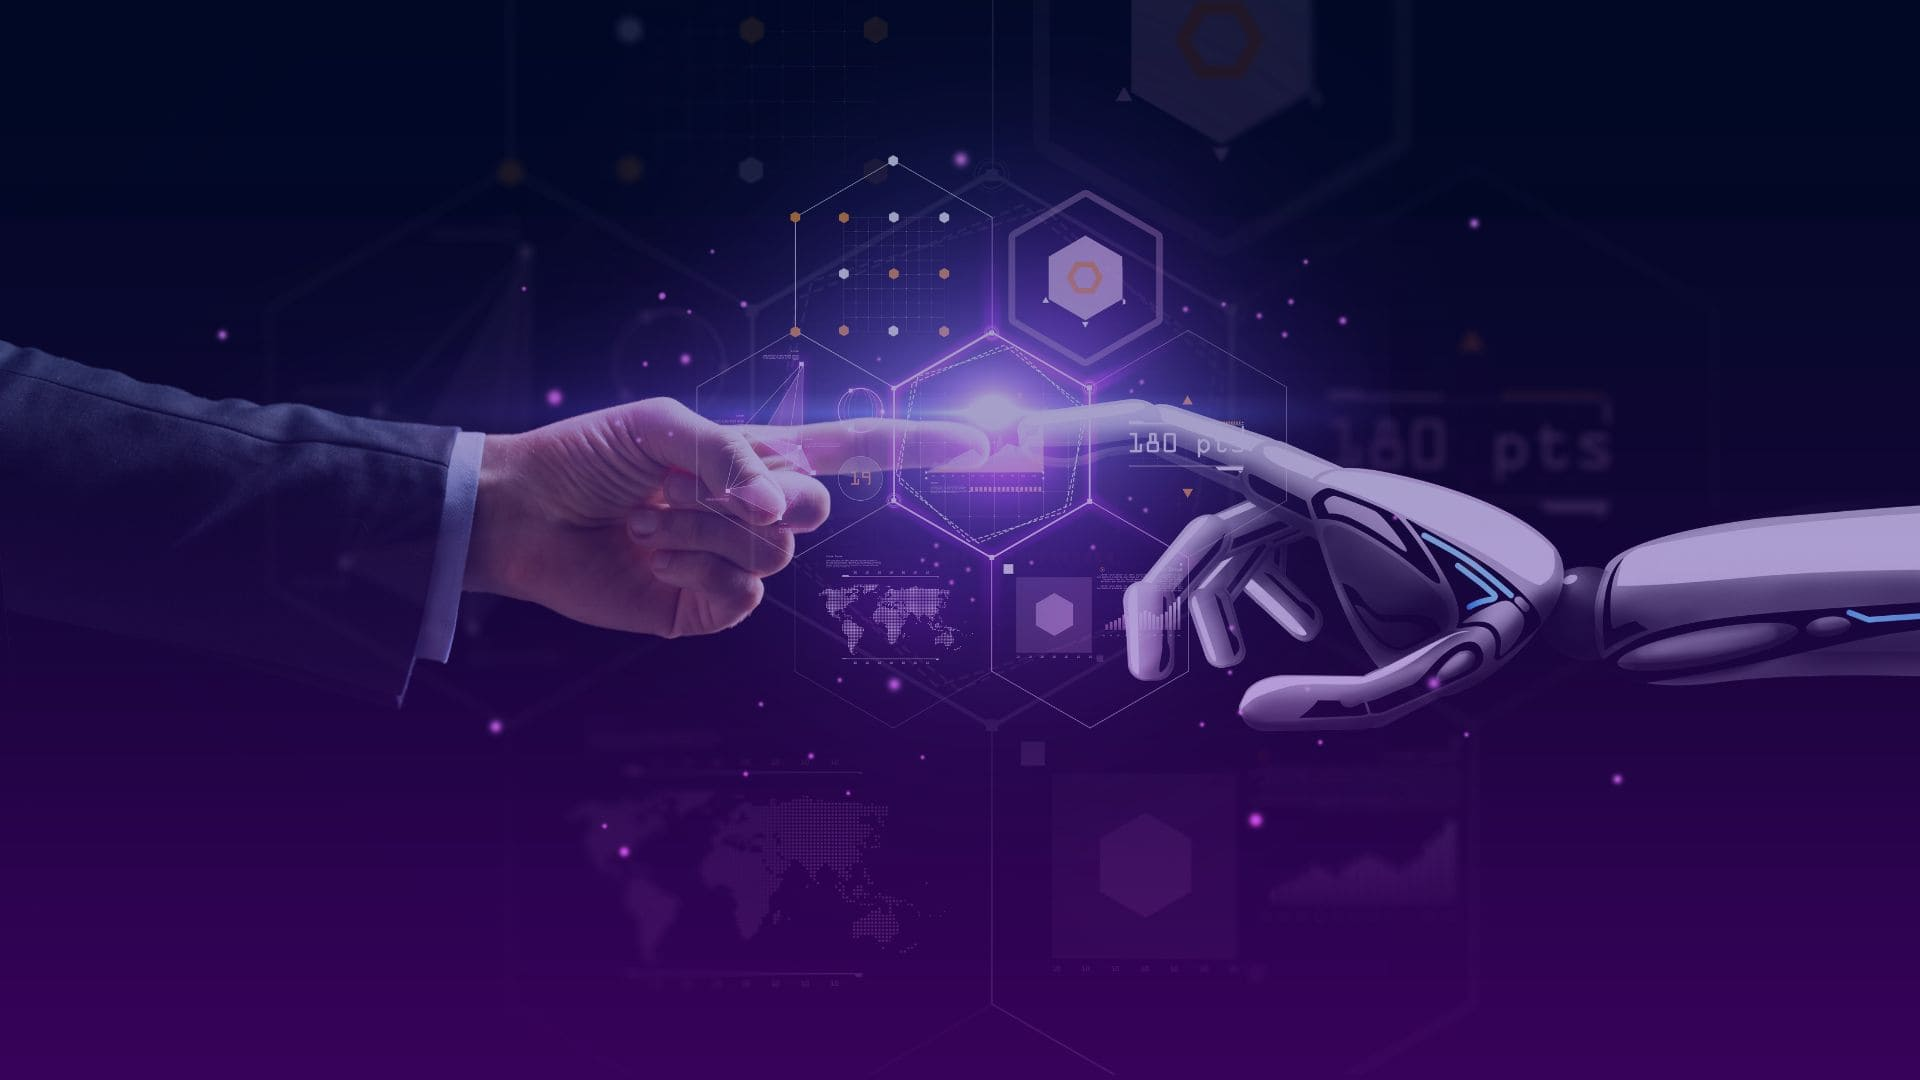
\includegraphics[width=\paperwidth,height=\paperheight]{images/capa.jpg}
}
	

\begin{frame}

\end{frame}
}


%% Titulo

{
\usebackgroundtemplate{
\centering

\includegraphics[width=\paperwidth,height=\paperheight]{images/fundo.pdf}
}
	
% Frame 3: plano de fundo
\begin{frame}
\maketitle
	
\end{frame}
}

{
\usebackgroundtemplate{
\centering

\includegraphics[width=\paperwidth,height=\paperheight]{images/fundo.pdf}
}

\begin{frame}
	\centering
	\frametitle{\textcolor{blue}{Sumário}}
    %\large
	\setbeamercolor{section in toc}{fg=blue,bg=blue}
    \tableofcontents[currentsection,sectionstyle=show/shaded,subsectionstyle=show/show/shaded]
\end{frame}

}








\section{Introdu\c{c}ão} 

{
	\usebackgroundtemplate{
		\centering
		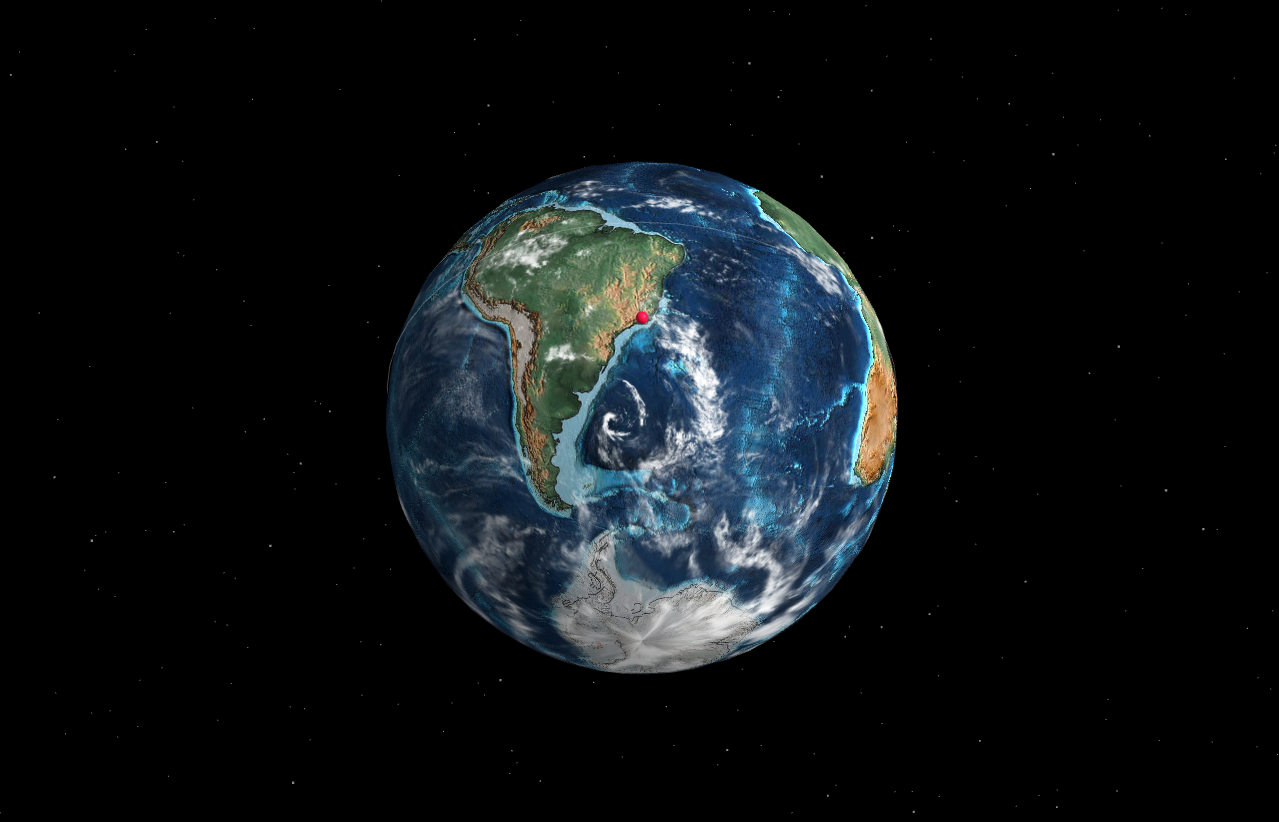
\includegraphics[width=\paperwidth,height=\paperheight]{images/holoceno.png}
	}
	
	% Frame 3: plano de fundo
	\begin{frame}
		\frametitle{\textcolor{yellow}{Olhemos para a Terra através de outra perspectiva...}}
\transboxin		


\flushright
\textcolor{yellow}{Tempo recente}
	\end{frame}
}


{
	\usebackgroundtemplate{
		\centering
		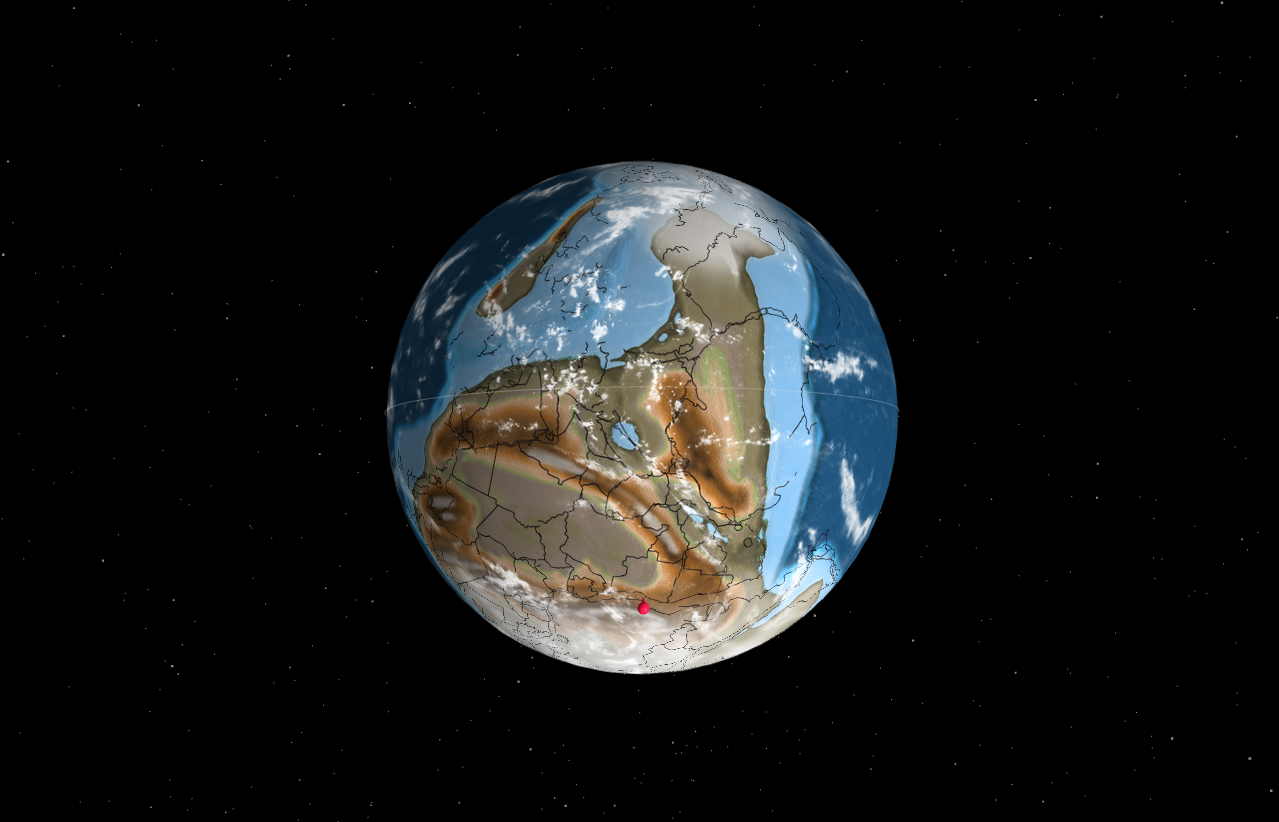
\includegraphics[width=\paperwidth,height=\paperheight]{images/ediacariano.png}
	}
	
	% Frame 3: plano de fundo
	\begin{frame}
		\frametitle{\textcolor{yellow}{E voltemos um pouco ao passado, no Ediacariano...}}
\transboxout	

\flushright
\textcolor{yellow}{$\pm$575 Ma atrás}
	\end{frame}
}


{
	\usebackgroundtemplate{
		\centering
		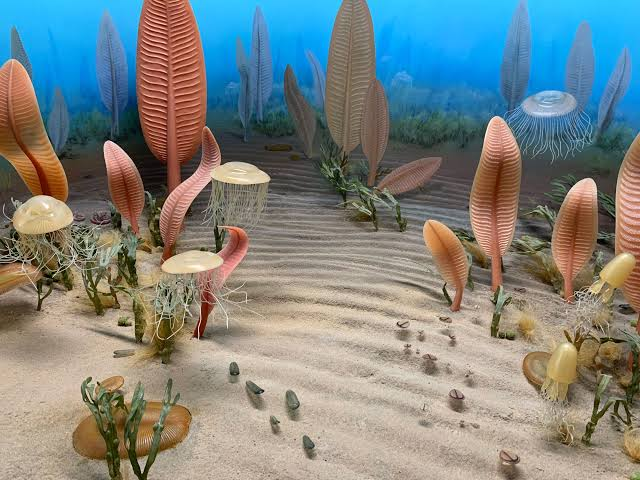
\includegraphics[width=\paperwidth,height=\paperheight]{images/faunaediacarana.jpeg}
	}
	
	% Frame 3: plano de fundo
	\begin{frame}
		\frametitle{\textcolor{yellow}{A vida diversifica-se nos oceanos}}
	\transdissolve	
	\end{frame}
}

{
	\usebackgroundtemplate{
		\centering
		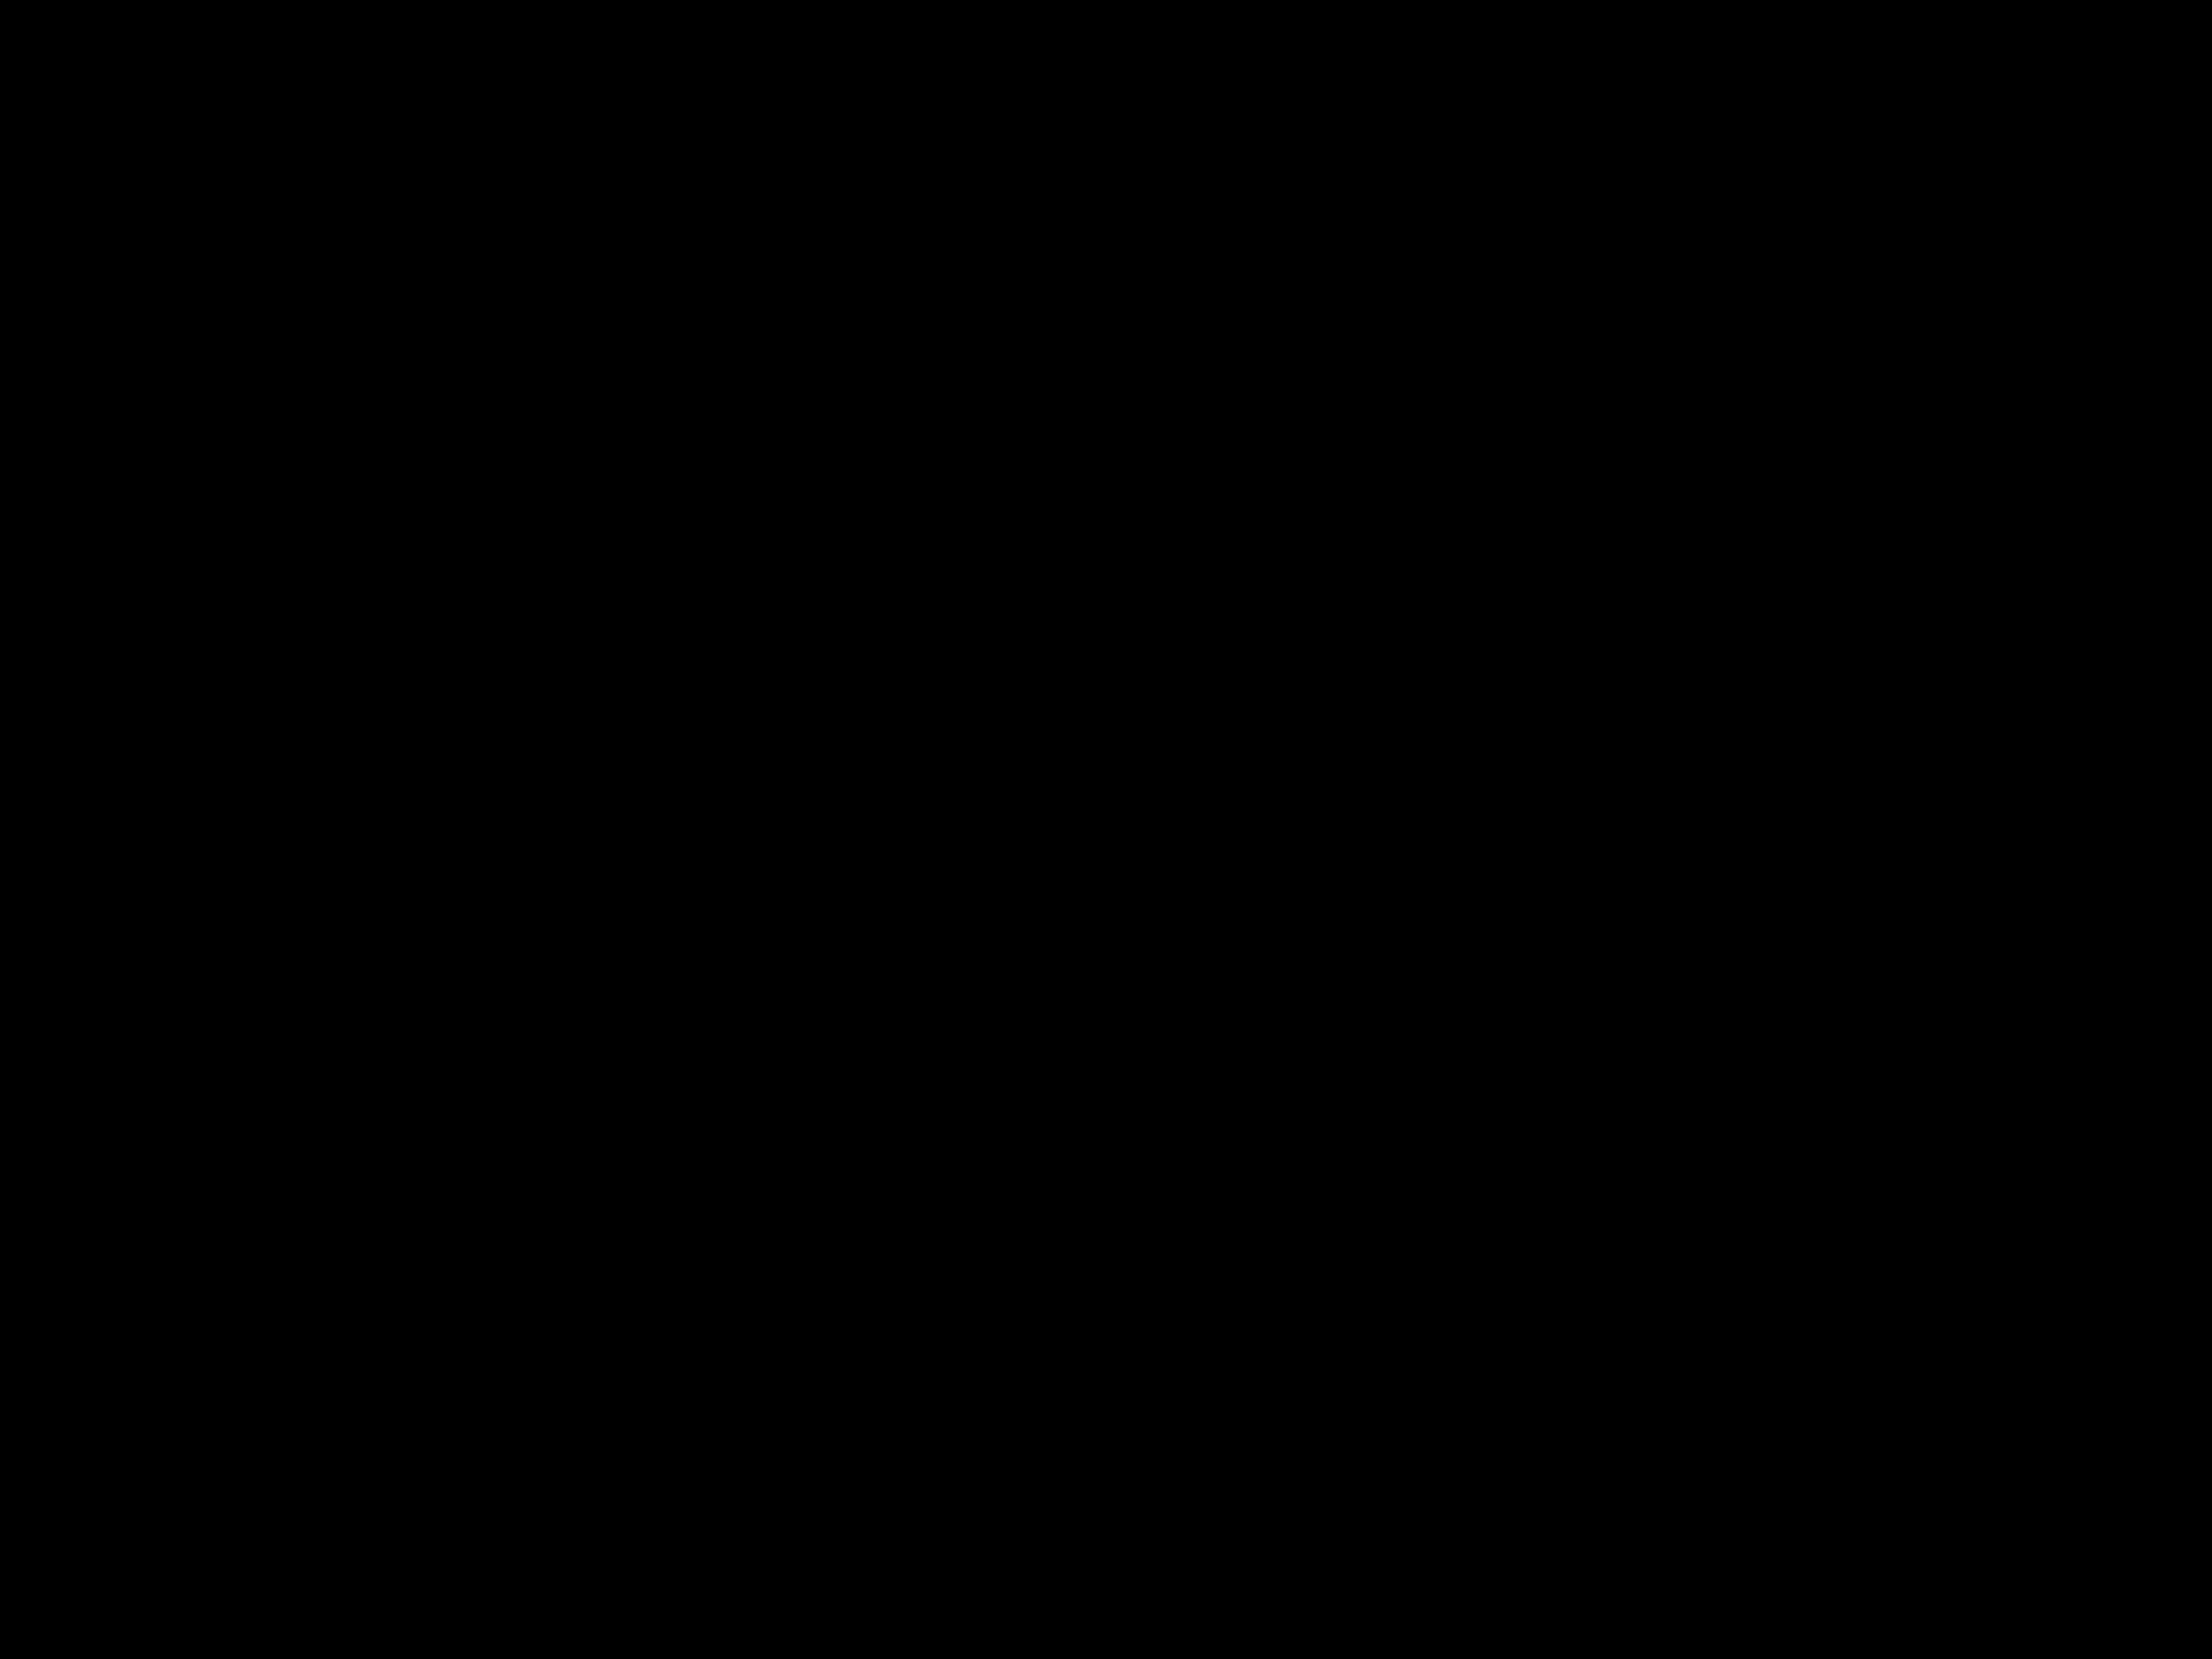
\includegraphics[width=\paperwidth,height=\paperheight]{images/fundopreto.png}
	}
	
	% Frame 3: plano de fundo
	\begin{frame}
		\frametitle{\textcolor{yellow}{Registros da Fauna de Ediacara}}
	\transboxout	
    
    \begin{minipage}{0.5\textwidth}
	    \begin{figure}
	\centering
        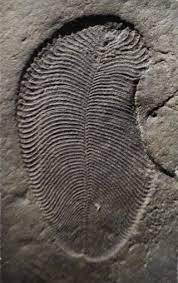
\includegraphics[scale=0.3]{images/faunaediacara3.jpeg} % Substitua pelo caminho da sua primeira figura
		    \caption{\textcolor{white}{\textit{Dickinsonia costata}, é um dos registros fósseis mais comum desse tempo.}} % Opcional
	    \end{figure}
    \end{minipage}%
		\pause
    \begin{minipage}{0.5\textwidth}
	    \begin{figure}
        \centering
        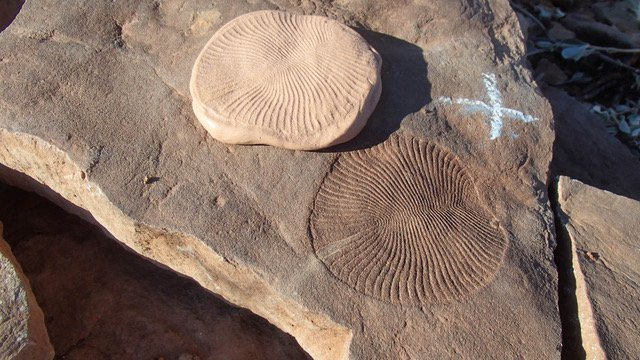
\includegraphics[scale=0.25]{images/faunaediacaran2.jpg} % Substitua pelo caminho da sua segunda figura
		    \caption{\textcolor{white}{Deslocava-se entre o sedimento de fundo, geralmente areias finas. Este espécime tinha cerca  de 6 centímetros de diâmtetro e fora encontrado, no sul da Austrália, e se alimentavam de tapetes microbialinos.}} % Opcional
	    \end{figure}
    \end{minipage}

\flushright
		\textcolor{blue}{\citep{Droser2024}}
		
	\end{frame}
}






{
	\usebackgroundtemplate{
		\centering
		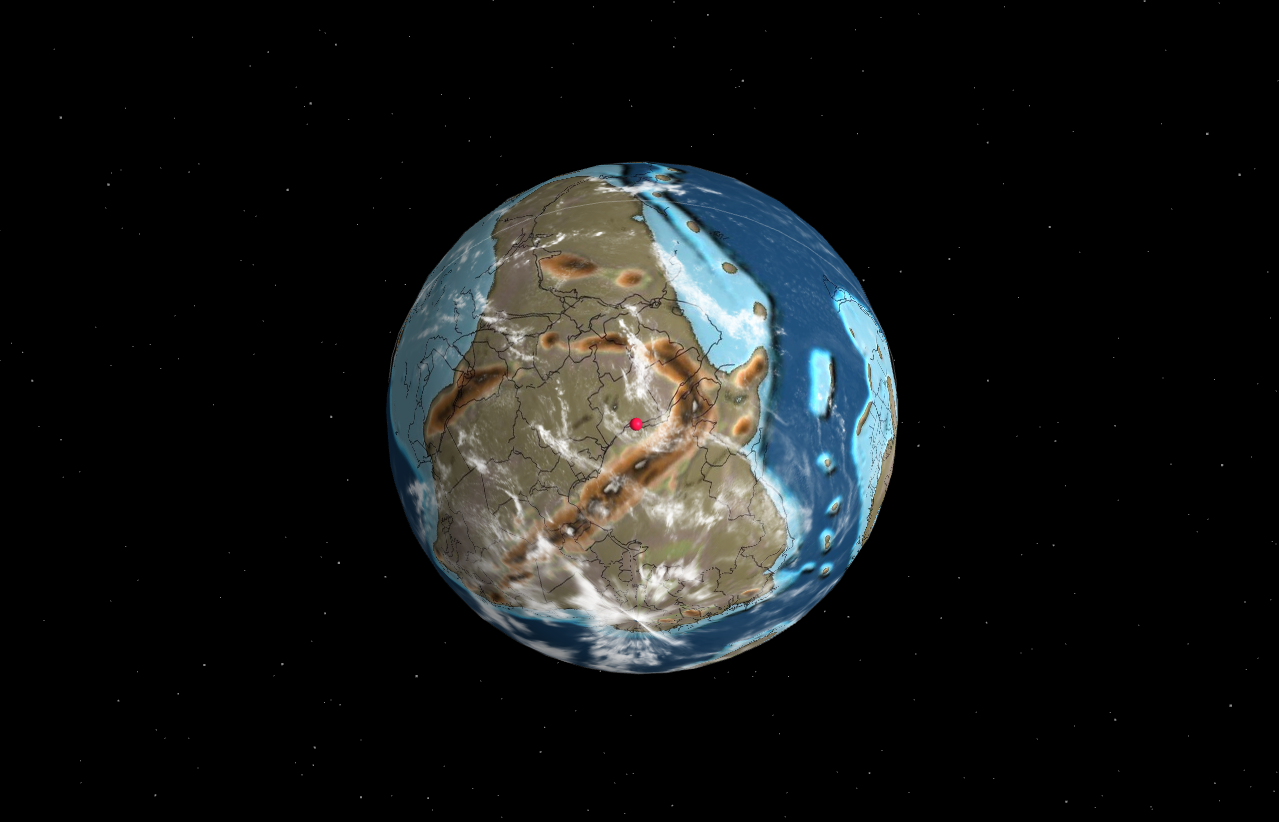
\includegraphics[width=\paperwidth,height=\paperheight]{images/cambriano.png}
	}
	
	% Frame 3: plano de fundo
	\begin{frame}
		\frametitle{\textcolor{yellow}{Avancemos um pouco mais, no tempo ...}}
	\transdissolve	
	
	\flushright
	\textcolor{yellow}{$\pm$505 Ma atrás}


\end{frame}
}




{
	\usebackgroundtemplate{
		\centering
		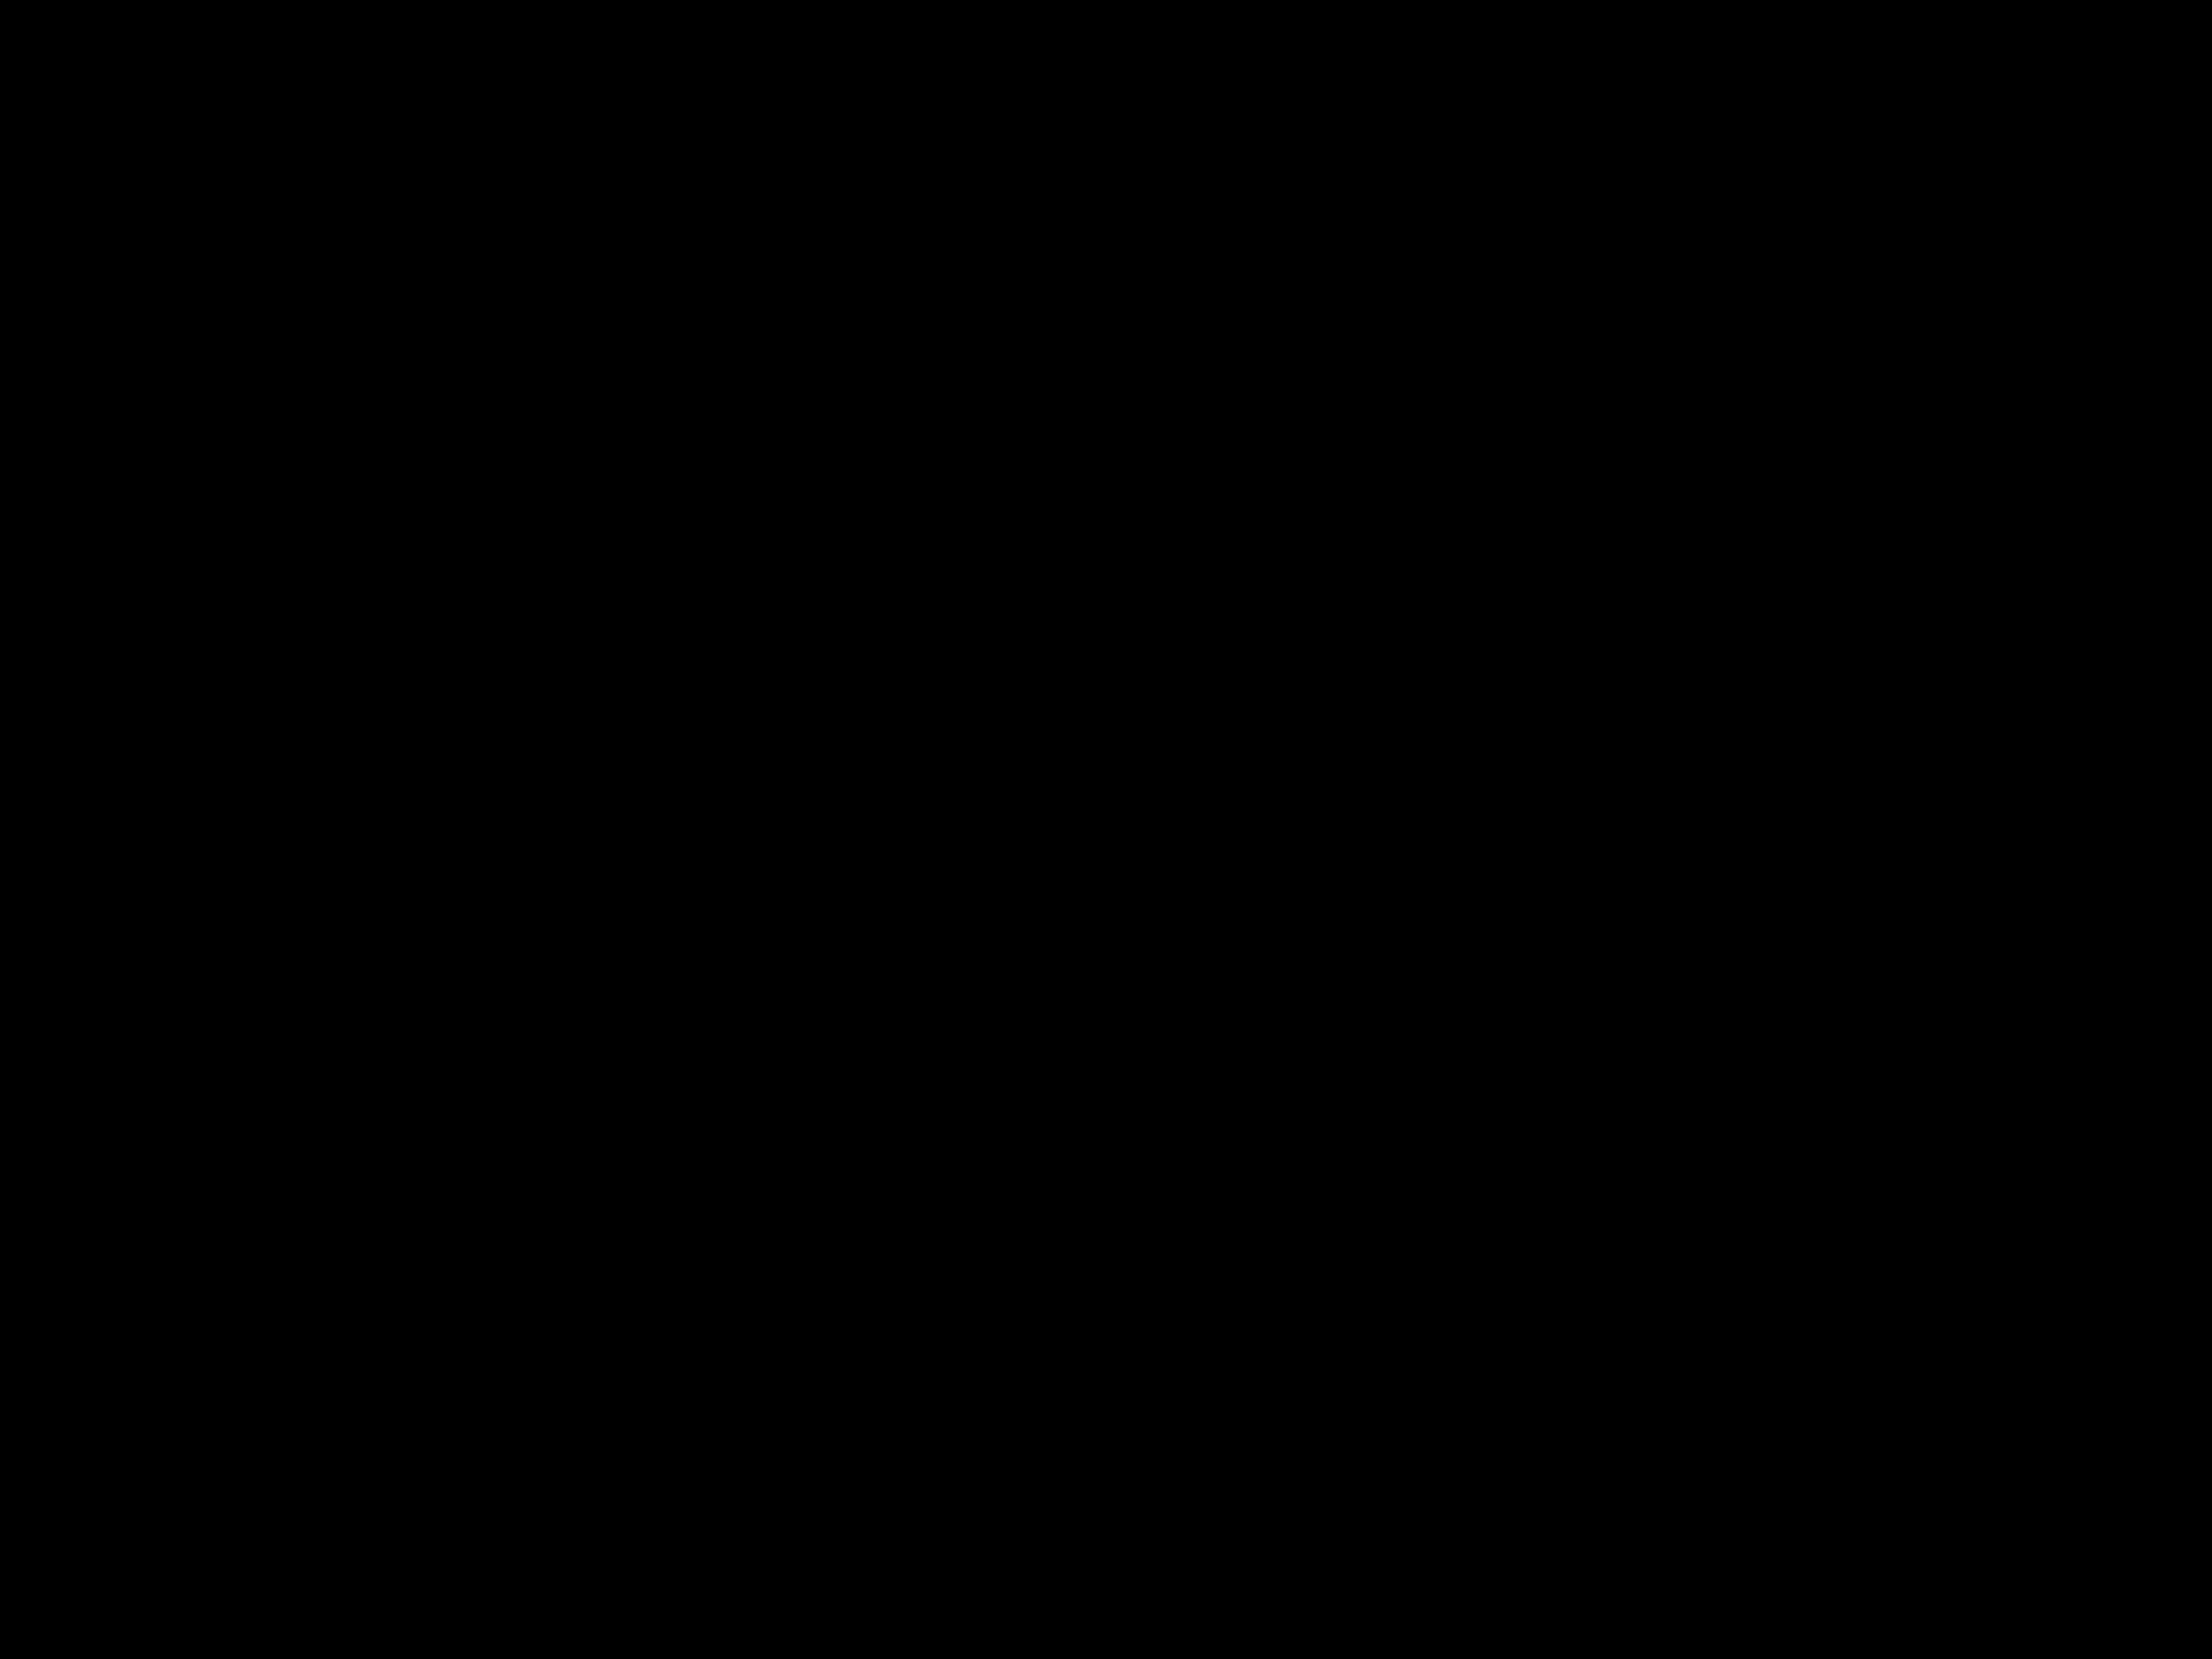
\includegraphics[width=\paperwidth,height=\paperheight]{images/fundopreto.png}
	}
	
	% Frame 3: plano de fundo
	\begin{frame}
		\frametitle{\textcolor{yellow}{Registros da Fauna de Cambriana}}
	\transboxout	
    
    \begin{minipage}{0.5\textwidth}
	    \begin{figure}
	\centering
        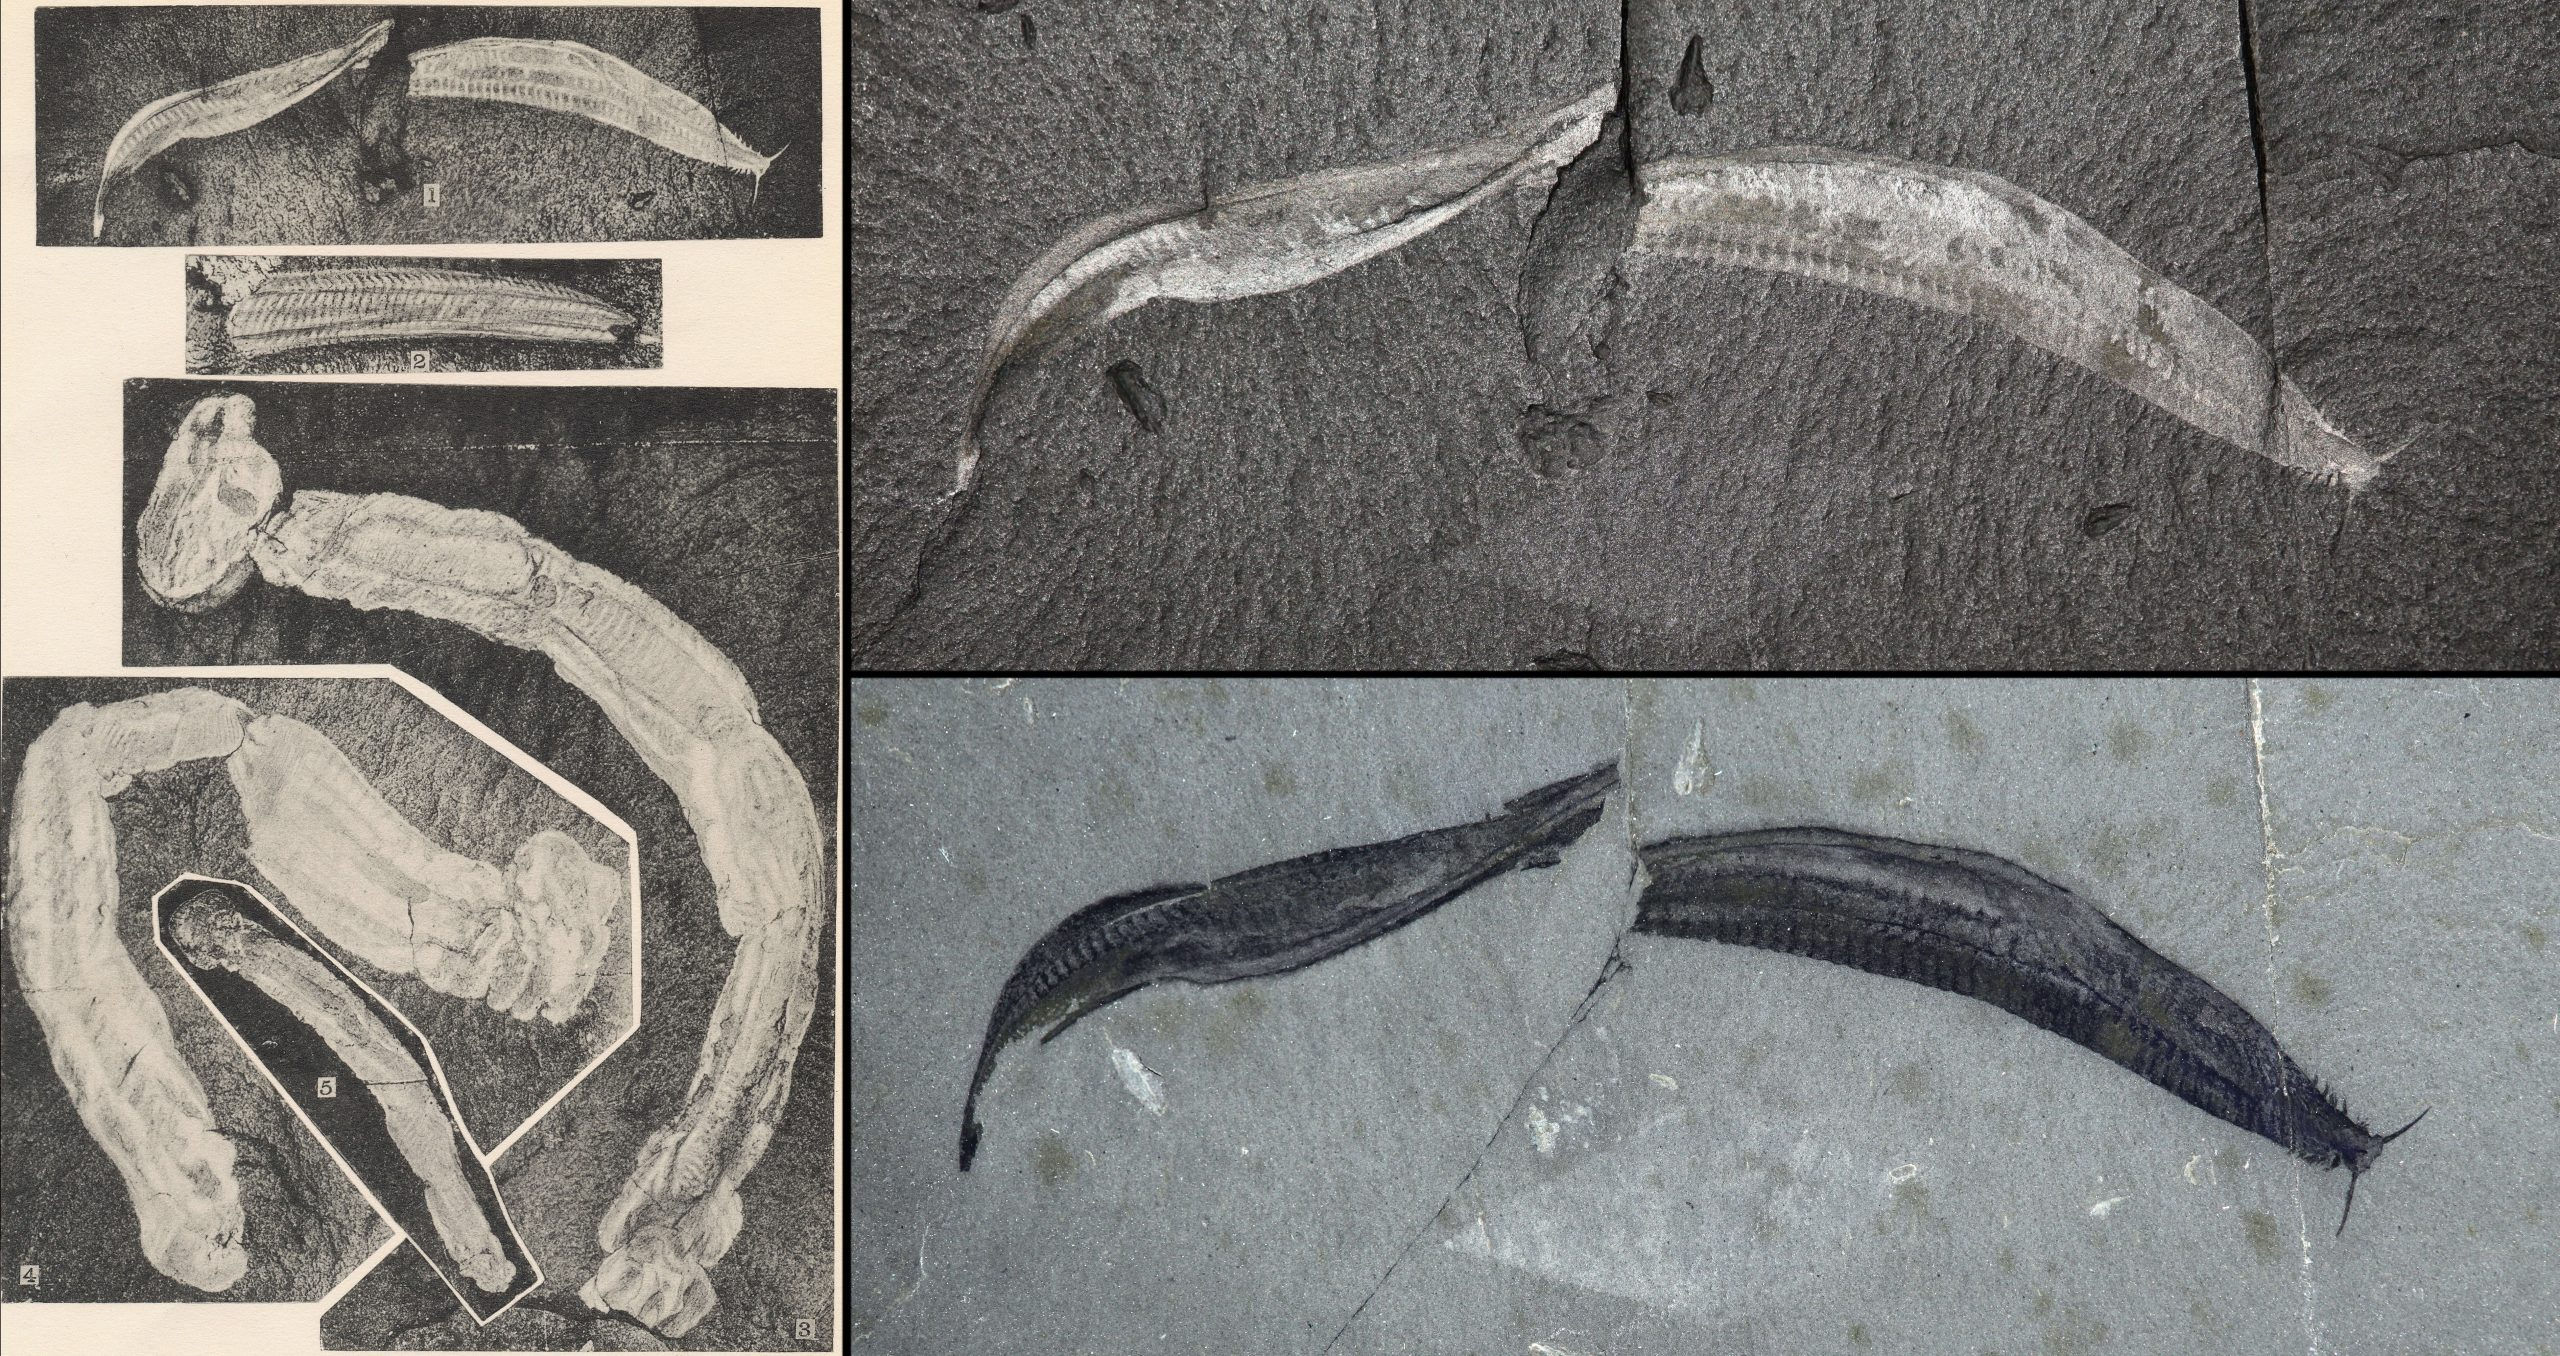
\includegraphics[scale=0.1]{images/faunacambriana3.jpg} % Substitua pelo caminho da sua primeira figura
		    \caption{\textcolor{white}{\textit{Pikaia gracilens}, é o fóssil mais notável desse tempo, representante dos primeiros cordatas com vasto registro no folhelho Burgess, no escudo Canadense.}} % Opcional
	    \end{figure}
    \end{minipage}%
		\pause
    \begin{minipage}{0.5\textwidth}
	    \begin{figure}
        \centering
        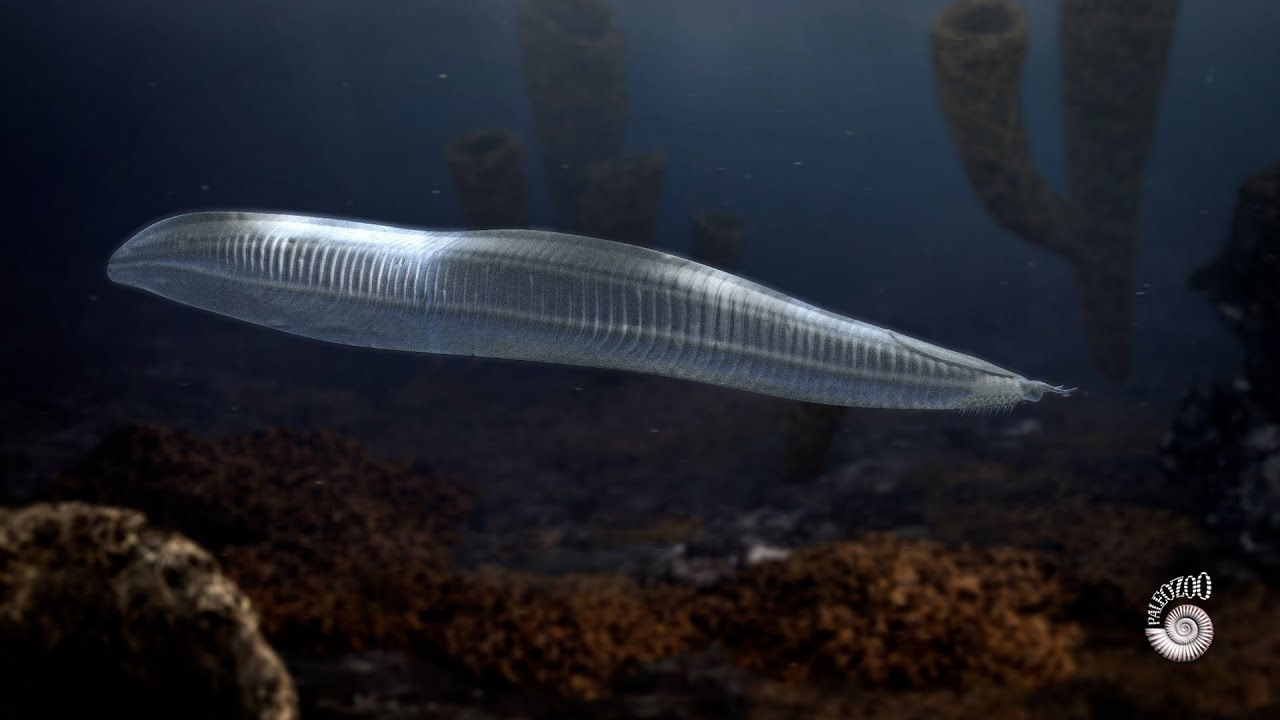
\includegraphics[scale=0.15]{images/faunacambriana2.jpg} % Substitua pelo caminho da sua segunda figura
		    \caption{\textcolor{white}{O corpo é lateralmente achatado com evidência de uma nadadeira ventral. Uma estrutura dorsal estreita que percorre o comprimento do organismo pode representar uma notocorda. Não possuem evidência de olhos.}} % Opcional
	    \end{figure}
    \end{minipage}

\flushright
		\textcolor{blue}{\citep{Briggs2015}}
		
	\end{frame}
}

{
	\usebackgroundtemplate{
		\centering
		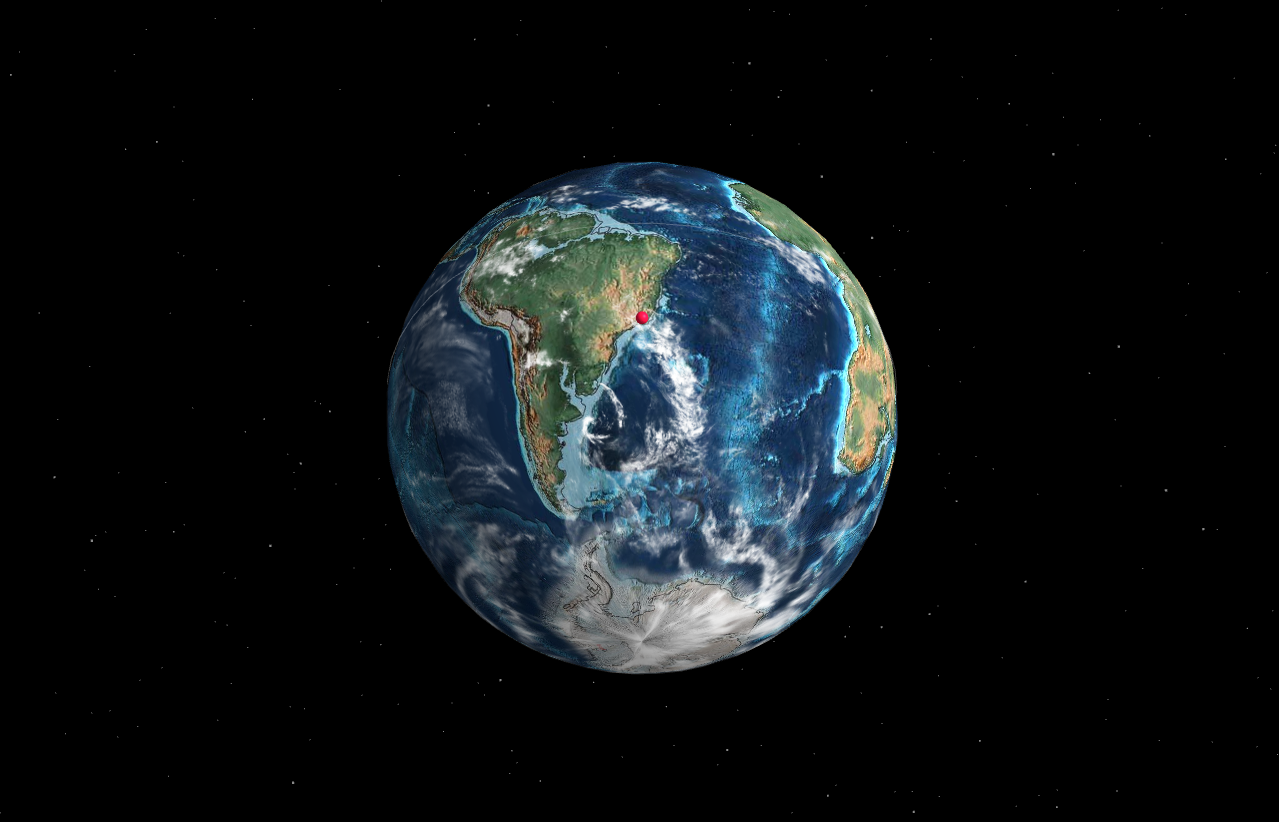
\includegraphics[width=\paperwidth,height=\paperheight]{images/neoceno.png}
	}
	
	% Frame 3: plano de fundo
	\begin{frame}
		\frametitle{\textcolor{yellow}{Agora vamos avançar bastante, no tempo ...}}
	\transdissolve	

	\flushright
    \textcolor{yellow}{$\pm$ 1.2 Ma atrás}
	\end{frame}
}


{
	\usebackgroundtemplate{
		\centering
		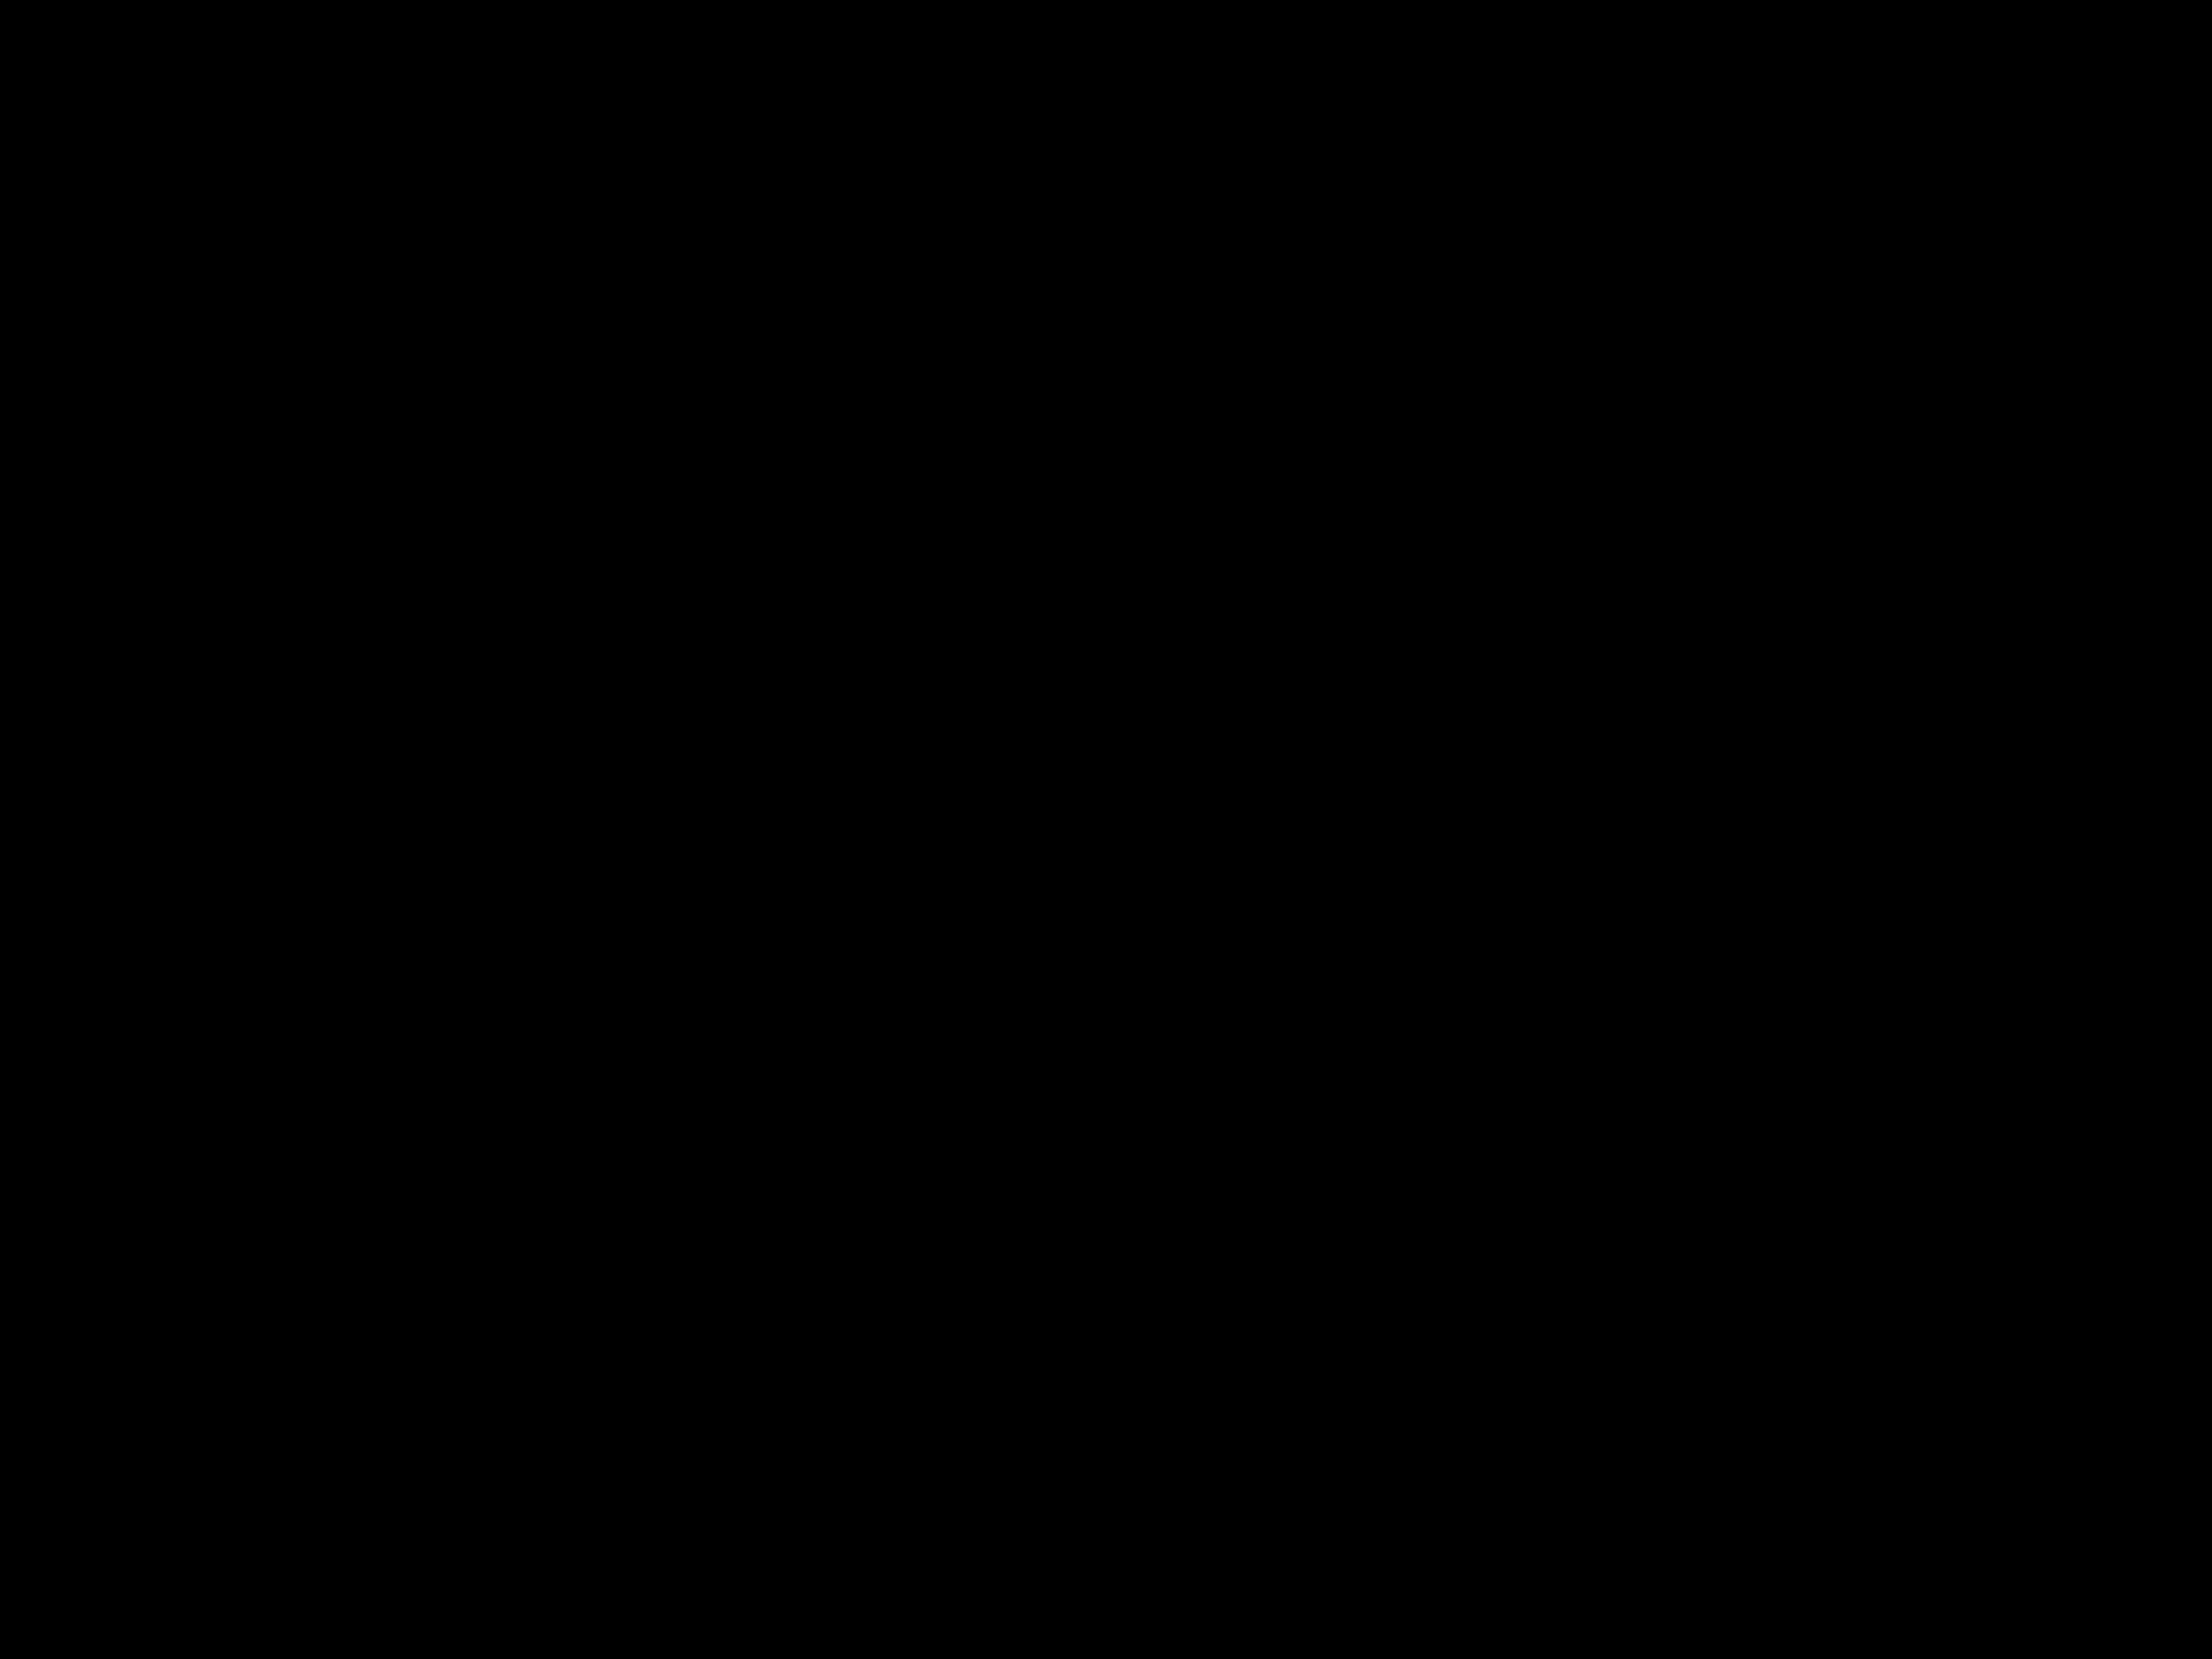
\includegraphics[width=\paperwidth,height=\paperheight]{images/fundopreto.png}
	}
	
	% Frame 3: plano de fundo
	\begin{frame}
		\frametitle{\textcolor{yellow}{Registros dos primeiros hominídeos}}
	\transboxout	
    
    \begin{minipage}{0.5\textwidth}
	    \begin{figure}
	\centering
        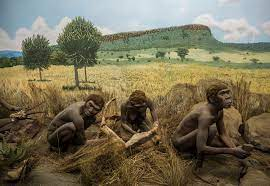
\includegraphics[scale=0.5]{images/australopitecus5.jpeg} % Substitua pelo caminho da sua primeira figura
		    \caption{\textcolor{white}{\textit{ Australopithecus anamensis}, fornece evidências sólidas do bipedismo a cerca de 3.9 Ma, na atual Etiópia.}} % Opcional
	    \end{figure}
    \end{minipage}%
		\pause
    \begin{minipage}{0.5\textwidth}
	    \begin{figure}
        \centering
        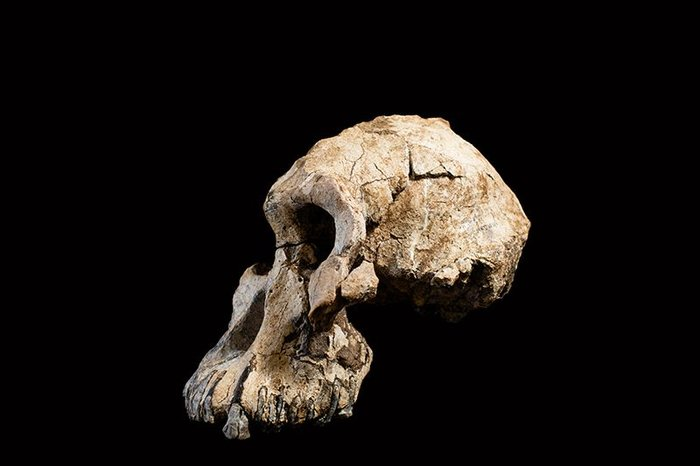
\includegraphics[scale=0.2]{images/australopitecus2.jpg} % Substitua pelo caminho da sua segunda figura
		    \caption{\textcolor{white}{Apesar de possuir andar bípede, eles tiveram braços longos. A relação do osso de braço superior (úmero) para osso de perna superior (fêmur) e está virtualmente igual ao de um Chimpanzé ($95\%$) do que um humano moderno ( $70\%$.) }} % Opcional
	    \end{figure}
    \end{minipage}

\flushright
		\textcolor{blue}{\citep{Higham2011}}
		
	\end{frame}
}

\section{Inteligência versus aprendizado}

\section{Trazendo o aprendizado para um computador}

\section{Conceitos envolvidos}

\section{O Perceptron e as demais RNAs}

\section{Mãos à obra}

\section{Um exemplo prático}
{
\usebackgroundtemplate{
\centering
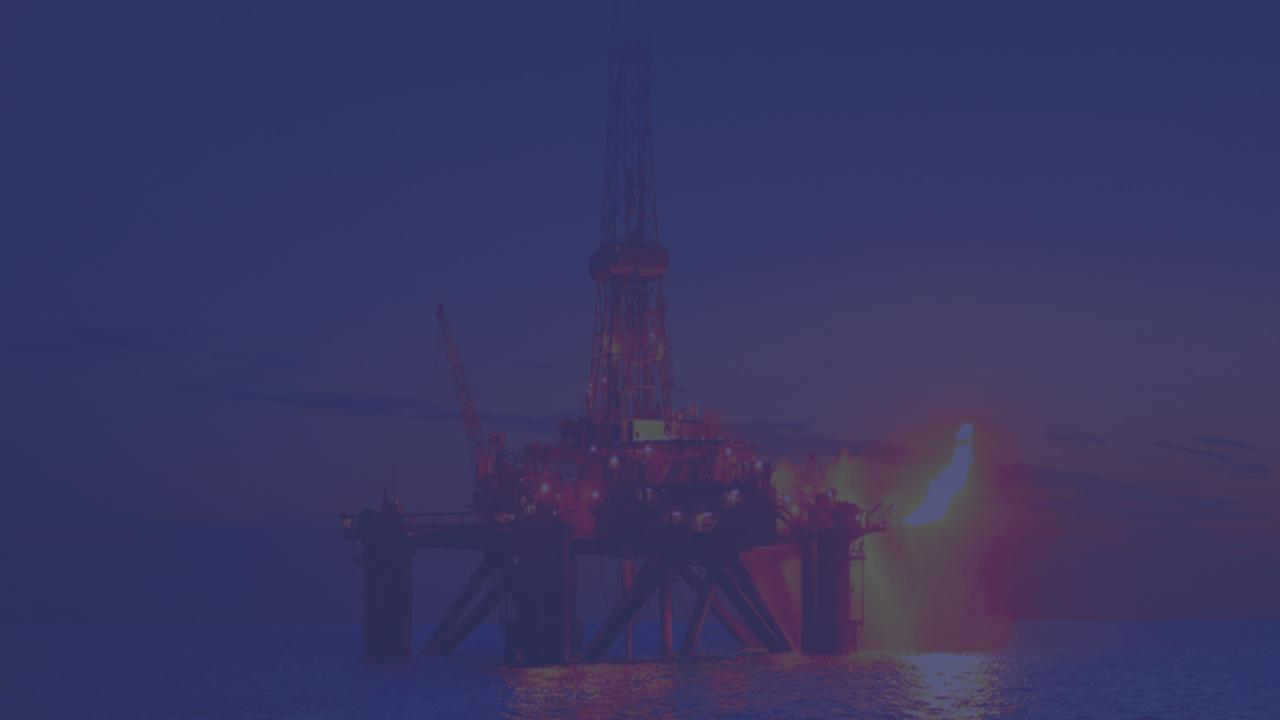
\includegraphics[width=\paperwidth,height=\paperheight]{images/fundonovo.jpg}
}
\begin{frame}
\vspace{2cm}
\begin{center}
\huge
	\textcolor{orange}{Um exemplo prático}
\end{center}

\end{frame} 
}


\section{Bate-papo}



















%%%%%%%%%%%%%%%%%%%%%%%%%%%%%%%%%%%%%%% REFERENCES %%%%%%%%%%%%%%%%%%%%%%%%%%%%%%%%%%%%%%%%%%%%%%%%%


{
\usebackgroundtemplate{
\centering

\includegraphics[width=\paperwidth,height=\paperheight]{images/fundo.pdf}
}
\begin{frame}[allowframebreaks]
\frametitle{Referências}
%\beamertemplatetextbibitems
\tiny
\bibliographystyle{apalike}
\bibliography{references.bib}

\end{frame}



\end{document}
